\documentclass[sigconf,nonacm]{acmart}
\settopmatter{printacmref=false, printccs=false, printfolios=true}
\setcopyright{none}
\acmDOI{}
\acmISBN{}
\acmConference{}{}{}
\acmYear{2026}
\copyrightyear{2026}
\usepackage{graphicx}
\usepackage{booktabs}
\usepackage{array}
\usepackage{balance}
\usepackage{xcolor}
\graphicspath{{figures/}}
\newcommand{\treat}[1]{\textbf{T#1}}
\begin{document}
\title{Shrinking Code: When Reuse Saves Lines but Costs More Generation Effort}
\author{Omar Dylan Abou}
\email{odabou@ncsu.edu}
\affiliation{\institution{North Carolina State University}\city{Raleigh}\state{NC}\country{USA}}
\author{Henoc Dossou}
\email{hbdossou@ncsu.edu}
\affiliation{\institution{North Carolina State University}\city{Raleigh}\state{NC}\country{USA}}
\author{Andrew Sergison}
\email{arsergis@ncsu.edu}
\affiliation{\institution{North Carolina State University}\city{Raleigh}\state{NC}\country{USA}}
\renewcommand{\shortauthors}{Abou, Dossou, and Sergison}
\begin{abstract}
Does code reuse reduce the source needed to deliver a suite of related software-engineering and AI tasks? We study ten car-inventory skills on Auto93 under six Claude-generated conditions that vary library availability and whether implementations share a growing codebase. Four independent V2 generation repetitions (240 planned skill outcomes) were evaluated against a frozen acceptance protocol. Of these, 221 passed, five failed competency checks, nine failed syntax generation, and five were blocked by earlier failures. In all five matched pairs where both compared implementations completed ten skills, reuse reduced physical source lines, but the reuse variants required more generation time and estimated API-equivalent dollars in every Python and scikit-learn repetition. A seventh, AI-assisted coursework-reuse implementation passed ten local checks but is not an unaided human baseline. The evidence supports a source-size tradeoff, not a statistically ranked seven-way winner.
\end{abstract}
\keywords{code reuse, generated software, experimental software engineering, lines of code, repeated trials}
\maketitle

\section{Question and Study Design}
A used-car client wants ten abilities: \emph{remember, guess, certify, flow, blame, justify, choose, fix, spot}, and \emph{race}. The tasks span inventory ranking, prediction, significance testing, streaming change detection, diagnosis, explanations, budgeted selection, hypothetical repair, anomaly detection, and search comparison. Each corresponds to two customer requirements in the project specification. The dataset is Auto93 (398 cars), split into 318 training and 80 held-out rows. Training-only statistics and masked test goals are required where applicable.

Our primary question is whether extending a reusable implementation needs fewer new lines than writing each skill separately. A secondary question is whether reduced source size also reduces implementation cost, time, or errors. We distinguish \emph{final physical LOC} (the accumulated standalone files versus the final shared program) from \emph{gross LOC added} across development steps. These are not identical measures.

\treat{1} and \treat{2} use plain Python without and with reuse; \treat{3} and \treat{4} similarly allow scikit-learn; \treat{5} and \treat{6} similarly allow EZR. Library availability is not enforced library use. The model, customer tasks, split, and V2 acceptance contracts were fixed for the four comparable independent generations R02--R05. For reuse, successive prompts extend one program and require earlier features to remain correct; without reuse, each skill is a standalone program. We retain generation failures instead of repairing outputs post hoc. R01 used a different contract and is excluded; the later incomplete R06 is also excluded from this analysis.

A seventh condition, \treat{7}, adapts existing EG5 and EG6 coursework using a 437-line, \emph{AI-assisted} adapter. It is a separately observed proof of coursework reuse (one implementation), not the human-only treatment anticipated by the original design. We therefore do not merge its development effort or runtime into the Claude treatment distributions.

\section{Measurements and Evaluation}
For each of 24 Claude treatment-runs, we measure generated snapshots, competency checks, syntax and dependency failures, physical LOC, prompt/input and output tokens, estimated API-equivalent cost, and model generation wall time. Tests use the same frozen V2 criteria; reused implementations additionally undergo regression checking. Estimated cost comes from recorded token usage and rate assumptions and \emph{is not} the user's Claude subscription bill. For execution-time comparisons, the Claude programs ran in GitHub Actions containers, while \treat{7} was checked locally on macOS.

\begin{table}[t]
\caption{Frozen V2 outcomes. Each arm has 40 planned skills across four generation repetitions. ``Gen fail'' denotes invalid syntax, while ``Block'' denotes a downstream reuse step not generated.}
\label{tab:outcome}
\centering
\small
\begin{tabular}{@{}lrrrr@{}}
\toprule
Arm & PASS & Gen fail & Test fail & Block \\
\midrule
T1 Python / separate & 39 & 1 & 0 & 0 \\
T2 Python / reuse & 38 & 0 & 2 & 0 \\
T3 sklearn / separate & 36 & 3 & 1 & 0 \\
T4 sklearn / reuse & 40 & 0 & 0 & 0 \\
T5 EZR available / separate & 34 & 4 & 2 & 0 \\
T6 EZR available / reuse & 34 & 1 & 0 & 5 \\
\midrule
Total & \textbf{221} & 9 & 5 & 5 \\
\bottomrule
\end{tabular}
\end{table}

\section{Results}
\subsection{Competency and completion}
Of the 240 planned outcomes, \textbf{221 passed (92.1\%)}. The 19 others comprise five test failures, nine syntax failures, and five blocked steps (Table~\ref{tab:outcome}). The strongest observed pass count is \treat{4} at 40/40; this is descriptive, not statistical proof of a universally superior treatment. A run with a syntax failure can still pass the remaining standalone skills, whereas an early failure in a reuse chain can prevent subsequent skills entirely.

\subsection{Final source size}
Figure~\ref{fig:loc} shows every \emph{matched, complete} ten-skill LOC comparison: three Python pairs (R02, R04, R05) and two scikit-learn pairs (R02, R03). All five favor reuse. Python's matched reductions were 38.4\%, 39.6\%, and 37.2\%; scikit-learn's were 40.1\% and 44.6\%. These are promising but small conditional samples, which exclude unsuccessful full builds. There is no complete matched EZR pair: no \treat{5} repetition generated all ten required standalone programs. Comparing a partly built codebase with a finished one would unfairly make the incomplete treatment look smaller.

\begin{figure}[t]
\centering
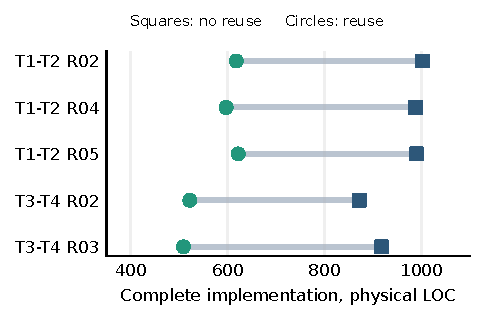
\includegraphics[width=\linewidth]{paired_LOC.pdf}
\Description{Five paired LOC results, all showing lower final source lines for reuse.}
\caption{Complete matched ten-skill LOC comparisons. Each line is one repetition comparing a no-reuse arm (square) to the corresponding reuse arm (circle).}
\label{fig:loc}
\end{figure}

\subsection{Tokens, cost, and wall time}
Across all 24 Claude treatment-runs, estimated API-equivalent generation cost was \textbf{\$15.81}. Figure~\ref{fig:cost} reports the upper median (the higher middle observation when $n=4$) cost per arm across attempted generations. In each of the four Python and four scikit-learn paired repetitions, the reuse treatment required more estimated dollars and more generation wall time. For example, R02 Python went from 1,003 to 618 LOC, but from \$0.350 to \$0.801 and from 145 to 266 seconds of generation. The growing codebase must be supplied and processed repeatedly, a plausible contributor to additional tokens. This is a mechanism hypothesis, not an independently isolated cause. Low cost on an incomplete generation must not be treated as an efficiency win.

\begin{figure}[t]
\centering
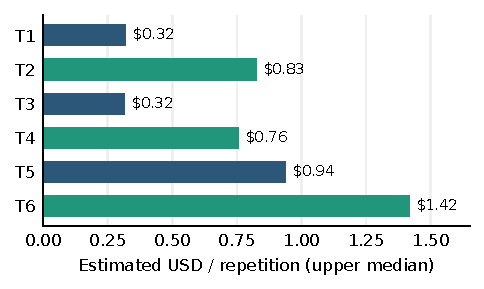
\includegraphics[width=\linewidth]{cost_median.pdf}
\Description{Upper-median estimated generation dollars are higher with reuse in the Python and sklearn pairs.}
\caption{Estimated API-equivalent USD per repetition (upper medians of attempted calls). Not normalized by skills successfully delivered.}
\label{fig:cost}
\end{figure}

\subsection{The T7-assisted observation}
The separately evaluated T7 adapter passed ten of ten local competency checkers once. It contains \textbf{437 new physical LOC}, plus 920 lines from EG5 and 580 from EG6, or 1,937 lines in the complete source footprint. These quantities cannot be substituted for one another. Selected task-level measurements include Guess MPG MAE of 4.275 (training-mean baseline 6.960), Choose inspecting 10 of 80 cars, and Spot F1 of 1.0 on 20 \emph{synthetically injected} anomalies. Flow's alert agreement was only 65.57\% despite passing interface/statistical checks. Race's adaptive mean best-at-ten quality was 0.1313 versus 0.1556 for random (lower is better). No independently timed human coding effort, API generation cost, or token accounting exists for this adapter.

\subsection{Task-level quality is not a pass count}
\begin{table}[t]
\caption{Selected task quality: upper medians for Claude arms among passing snapshots, versus one T7-assisted local observation. Lower is better for Guess MAE and Race best-at-ten; higher is better for Spot F1. Sample sizes and implementation conditions differ.}
\label{tab:quality}
\centering
\small
\begin{tabular}{@{}lrrr@{}}
\toprule
Arm & Guess MPG MAE & Spot F1 & Race best10 \\
\midrule
T1 & 3.998 & 1.000 & 0.1223 \\
T2 & 4.024 & 0.976 & 0.1159 \\
T3 & 3.359 & 0.952 & 0.1130 \\
T4 & 3.359 & 0.850 & 0.1130 \\
T5 & 3.983 & 0.976 & 0.1534 \\
T6 & 3.746 & 0.909 & 0.1139 \\
T7-assisted & 4.275 & 1.000 & 0.1313 \\
\bottomrule
\end{tabular}
\end{table}
A pass indicates meeting a defined competency contract, not dominance on every quality metric. For example, \treat{4} passed 40/40 skills, yet its upper-median Spot F1 was 0.850 on synthetic corruptions, compared with 1.000 for \treat{1}. Conversely, the scikit-learn conditions had lower observed MPG prediction error than plain Python in this sample. Table~\ref{tab:quality} provides complementary task-specific outcomes instead of claiming that these different measures form one overall score. Statistical comparison would also need to condition on the missing or unsuccessful programs and avoid pretending that one T7 output constitutes four independent samples.

\subsection{Why repetitions and skill-level outcomes matter}
\begin{table}[t]
\caption{Per-repetition accounting across six treatments, 60 outcomes per row. A full generation repetition may contain failed skill outcomes.}
\label{tab:reps}
\centering
\small
\begin{tabular}{@{}lrrrr@{}}
\toprule
Repeat & PASS & Syntax fail & Test fail & Block \\
\midrule
R02 & 53 & 2 & 0 & 5 \\
R03 & 53 & 2 & 5 & 0 \\
R04 & 58 & 2 & 0 & 0 \\
R05 & 57 & 3 & 0 & 0 \\
\bottomrule
\end{tabular}
\end{table}
The total passing fraction conceals different failure mechanisms (Table~\ref{tab:reps}). R02 had an early T6 reuse-chain syntax failure: five later steps were never generated and therefore cannot be assigned zero runtime or presented as individually tested failures. R03 had five actual competency-test failures among syntactically generated programs. R04 and R05, by contrast, failed only at generation syntax. This separation matters because a binary success indicator by itself would conflate three distinct events: rejection by the parser, incorrect behavior on the specified contract, and absence of a program due to a predecessor's failure.

The evaluation archive also preserves skill-level quality metrics, which are richer than PASS. For example, Guess was compared against an MPG training-mean baseline, Spot was scored by precision/recall on controlled corruptions, and Race compared adaptive and random selection under the same ten-label budget. A valid prediction output does not imply optimal error; similarly, a valid Flow implementation can agree with observed change labels only imperfectly. We treat such scores as domain-specific observations, not interchangeable dimensions of a single software ``quality'' number.

Finally, repetitions are independent \emph{code-generation paths}, not repeated stochastic search episodes on an unchanged generated file. Race's twenty episodes assess a \emph{single program}'s search behavior; they cannot be used to inflate the number of independent Claude builds from four to eighty. We retain the four generation identities when interpreting the source and generation-cost metrics. The paired reuse comparisons use the same repetition identifier, but no causal claim follows without accounting for task interfaces, prompt-context accumulation, and failure-related missingness.

\balance
\section{Statistical Interpretation and Limitations}
The course's \texttt{same()} method requires agreement among mean effects (Cohen $\leq0.35$), rank effects (absolute Cliff's delta $\leq0.195$), and distribution shape (scaled KS $\leq1.36$); \texttt{ranks()} then groups treatments with tied best ranks~\cite{gloss6}. These are effect/shape comparisons, not proof of equal methods. Our analysis pipeline withholds group ranks with fewer than five samples per arm. Here all Claude arms have only four generations, complete-LOC samples are smaller still, and T7 has only one observation. Accordingly, we report \emph{no} seven-way rank or significance claim. As exploratory diagnostics only, the T1/T2 estimated-cost samples yield Cohen 10.48, absolute Cliff's delta 1.00, and scaled KS 1.414; T3/T4 cost gives 9.58, 1.00, and 1.414. Thus neither pair meets the lecture's \texttt{same()} cutoffs on cost. With $n=4$ in each arm, these diagnostics do not establish a reliable treatment rank. The V2 \emph{Certify skill acceptance} uses a distinct Cliff threshold of 0.197; it must not be silently substituted for the lecture's 0.195 used in cross-treatment analysis.

Threats include a single data domain and split, acceptance tests that reward exact contract compliance rather than real-world utility, selective omission of failed full builds from LOC summaries, cached input-token and model-context effects, and nonidentical execution machines. The library labels also warrant care: the successful \treat{5}/\treat{6} snapshots did not directly import EZR, so those arms measure available context rather than demonstrated EZR calls. The human-only T7 control is \emph{not complete as specified}: AI assisted the adapter, and development time was not measured. It can be shown as an exploratory seventh condition only.

\section{Conclusion and Remaining Work}
Within complete, matched Python and scikit-learn implementations, reuse consistently shrank final source code, but it increased model generation time and estimated dollars. Correctness was high but not perfect and dependency-chain failures mattered. Next steps are to preserve this frozen record, report the missing T7 manual baseline honestly or carry out genuinely unaided, timed prudence checks, and add independent repetitions only if resources permit. The repository and final report should disclose protocols, code provenance, unresolved R06 infrastructure evidence, and all negative results. The progress-presentation slides are unaffected by this report.

\begin{thebibliography}{9}
\bibitem{gloss6} T. Menzies. 2026. A glossary of tiny lectures, part 6: statistics and ranking. \url{https://txt.github.io/seai26f/gloss6.html}.
\bibitem{cohen} J. Cohen. 1988. \emph{Statistical Power Analysis for the Behavioral Sciences}, 2nd ed. Lawrence Erlbaum.
\bibitem{cliff} N. Cliff. 1993. Dominance statistics: Ordinal analyses to answer ordinal questions. \emph{Psychological Bulletin} 114, 3, 494--509.
\bibitem{arcuri} A. Arcuri and L. Briand. 2011. A practical guide for using statistical tests to assess randomized algorithms in software engineering. \emph{ICSE}.
\end{thebibliography}
\end{document}
